\documentclass{beamer}
\usepackage{hyperref} % URLs
\title[Project management]{Effective project management }
%\subtitle[short]{full}
\author{Andy J. Wills}

\date{}

\begin{document}
%%%%% All images from wikimedia commons.

\frame{\titlepage}


\begin{frame}{Goals and sub-goals}
  \centerline{
  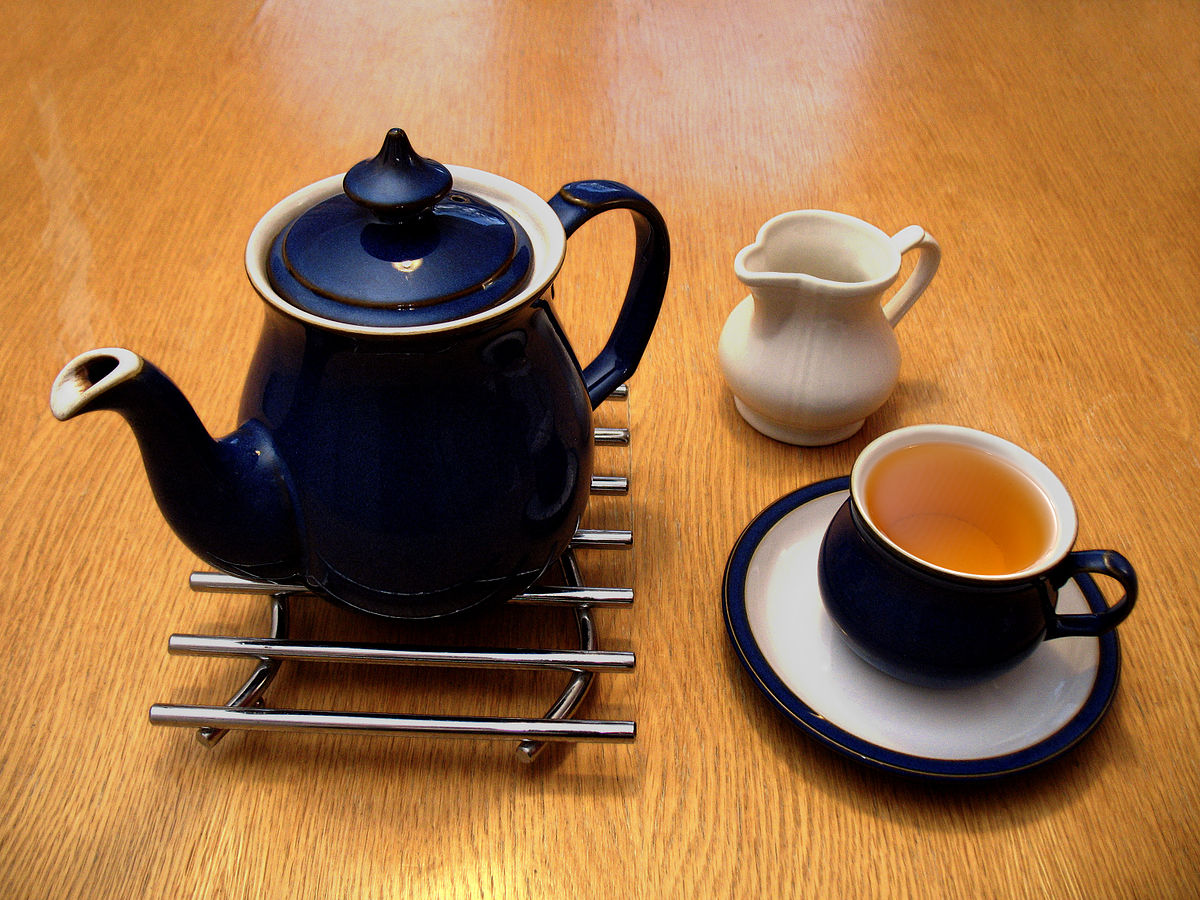
\includegraphics[width=.3\textwidth]{pics/Nice_Cup_of_Black_Tea.jpg}
}
  Making a cup of tea - breaking down into sub-goals.
  \begin{itemize}
    \item Boil water
 \item Get kettle
 \item Get cup
 \item Get tea bag
 \item Get milk
 \item Pour water on tea bag
 \item Add milk
  \end{itemize}
\end{frame}

\begin{frame}{Critical path analysis}
    \centerline{
  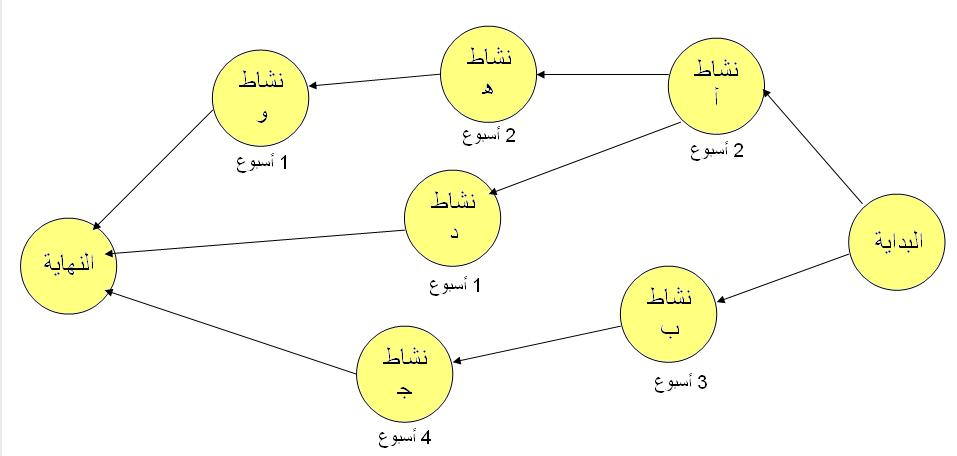
\includegraphics[width=.8\textwidth]{pics/Critical_path_diagram.JPG}
}
  What order do the sub-goals need to be achieved in?
  \begin{itemize}
    \item Get cup / get kettle / get tea bag
 \item Boil water
 \item Pour water on teabag
 \item Add milk
 \item Tea made!
  \end{itemize}
\end{frame}

\begin{frame}{Deadlines and sub-deadlines}
  \centerline{
  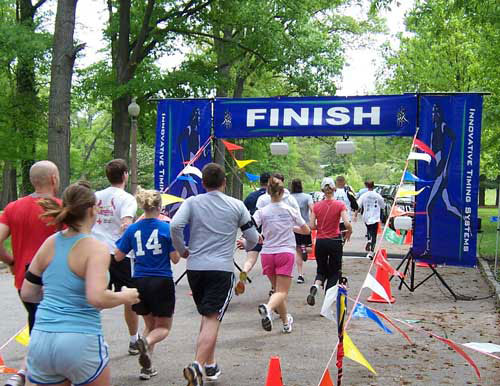
\includegraphics[width=.3\textwidth]{pics/Finish-SprintforSight-Large.jpg}
}
  
  Use final deadline, and time estimates, to set sub-deadlines.
  \begin{itemize}
    \item Get cup (7.49am) / get kettle (7.49am) / get tea bag (Monday 10pm)
    \item Boil water (7.50am)
    \item Pour water on teabag (7.55am)
    \item Add milk (7.59am 
    \item Tea made! (Tuesday 8am)
  \end{itemize}
\end{frame}

\begin{frame}{Scheduling your own time}
  \centerline{
  
\includegraphics[width=.3\textwidth]{pics/Eucalyp-Deus_Cocktail.png}
}

  
  Fitting around the rest of your life e.g. you're working Monday night.
  \begin{itemize}
    \item  Monday 2pm: Buy tea bags
 \item  Tuesday 7.49am: Get cup \& Kettle
 \item  7.50am: boil water
 \item  7.55am: Pour water on teabag
 \item  7.59am: Add milk 
 \item  8.00am: Tea made!
  \end{itemize}
\end{frame}

\begin{frame}{Assessment}
    \centerline{
  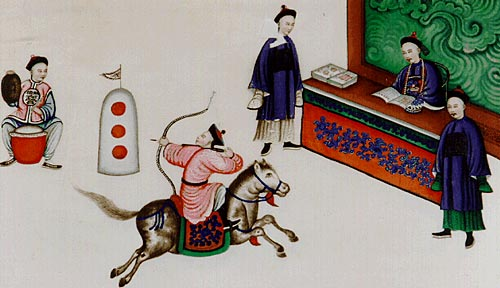
\includegraphics[width=.8\textwidth]{pics/Qing_military_exam_1.jpg}
}

  \begin{itemize}
    \item Write a schedule for your dissertation
    \item Agree with your supervisor
    \item Submit as PDF to Psyc:EL
  \end{itemize}
\end{frame}

\begin{frame}{Further study}
    \centerline{
  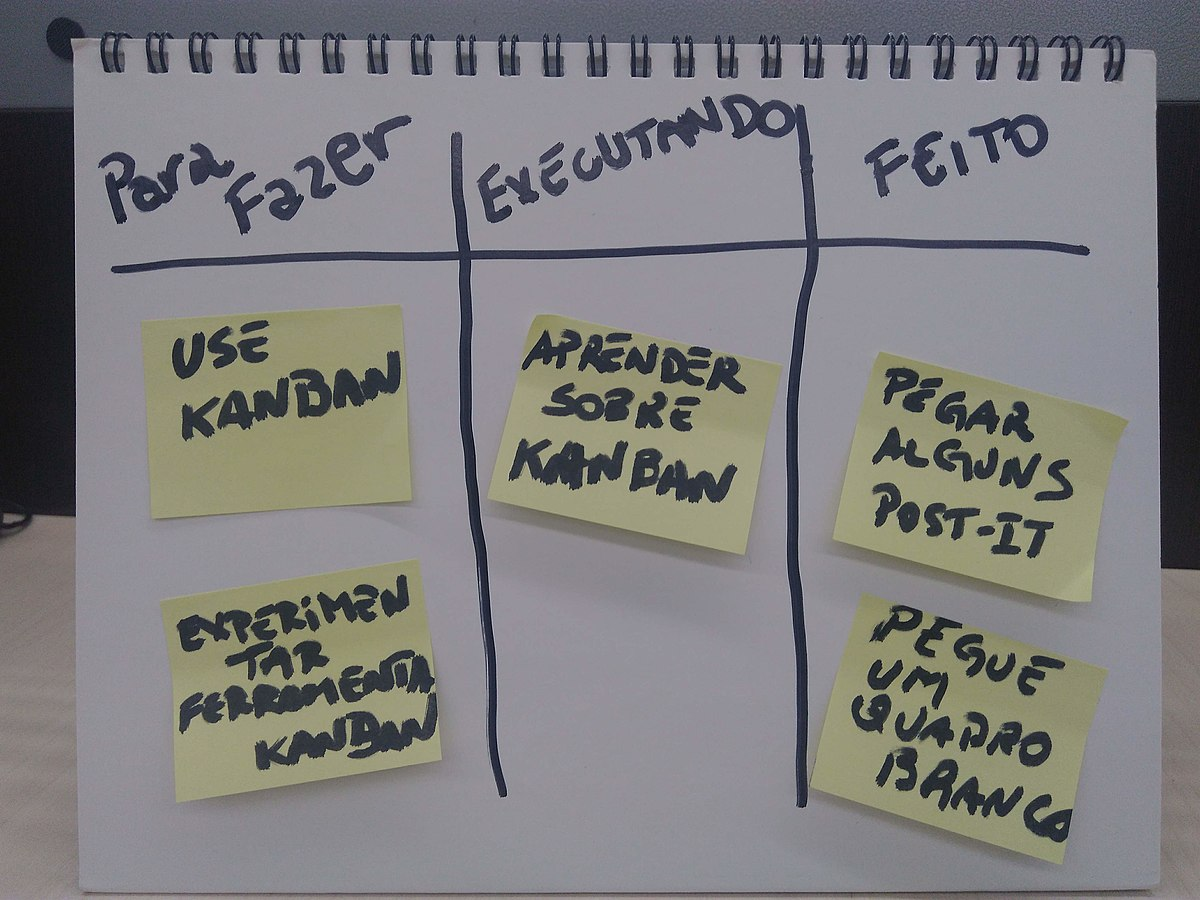
\includegraphics[width=.5\textwidth]{pics/Simples-Quadro-Kanban-03.jpg}
}
  
  \begin{itemize}
  \item Kanban is a technique for tracking the progress of a project
    \item Great materials at \url{https://www.atlassian.com/agile/kanban}
  \end{itemize}
\end{frame}

\tiny
This work is licensed under a Creative Commons Attribution-ShareAlike
4.0 International Licence. Last update: \today

\end{document}



%%% Local Variables:
%%% mode: latex
%%% TeX-master: t
%%% End:
